\subsection{Datapath architecture}
Per la realizzazione del datapath del processore è stato considerato come punto di partenza il processore descritto in \autoref{subsection:single_cycle} e in \autoref{subsection:pipe_arch} ed è stata derivata l'architettura presente in \autoref{fig:datapath_architecture}. Si nota come si è utilizzata sempre la suddivisione in cinque fasi e di conseguenza anche la pipeline. Inoltre è stato aggiunto nel design il register file ma non le memorie istruzioni e dati inserite soltanto in fase di testing.

\begin{figure}[h]
  \center
  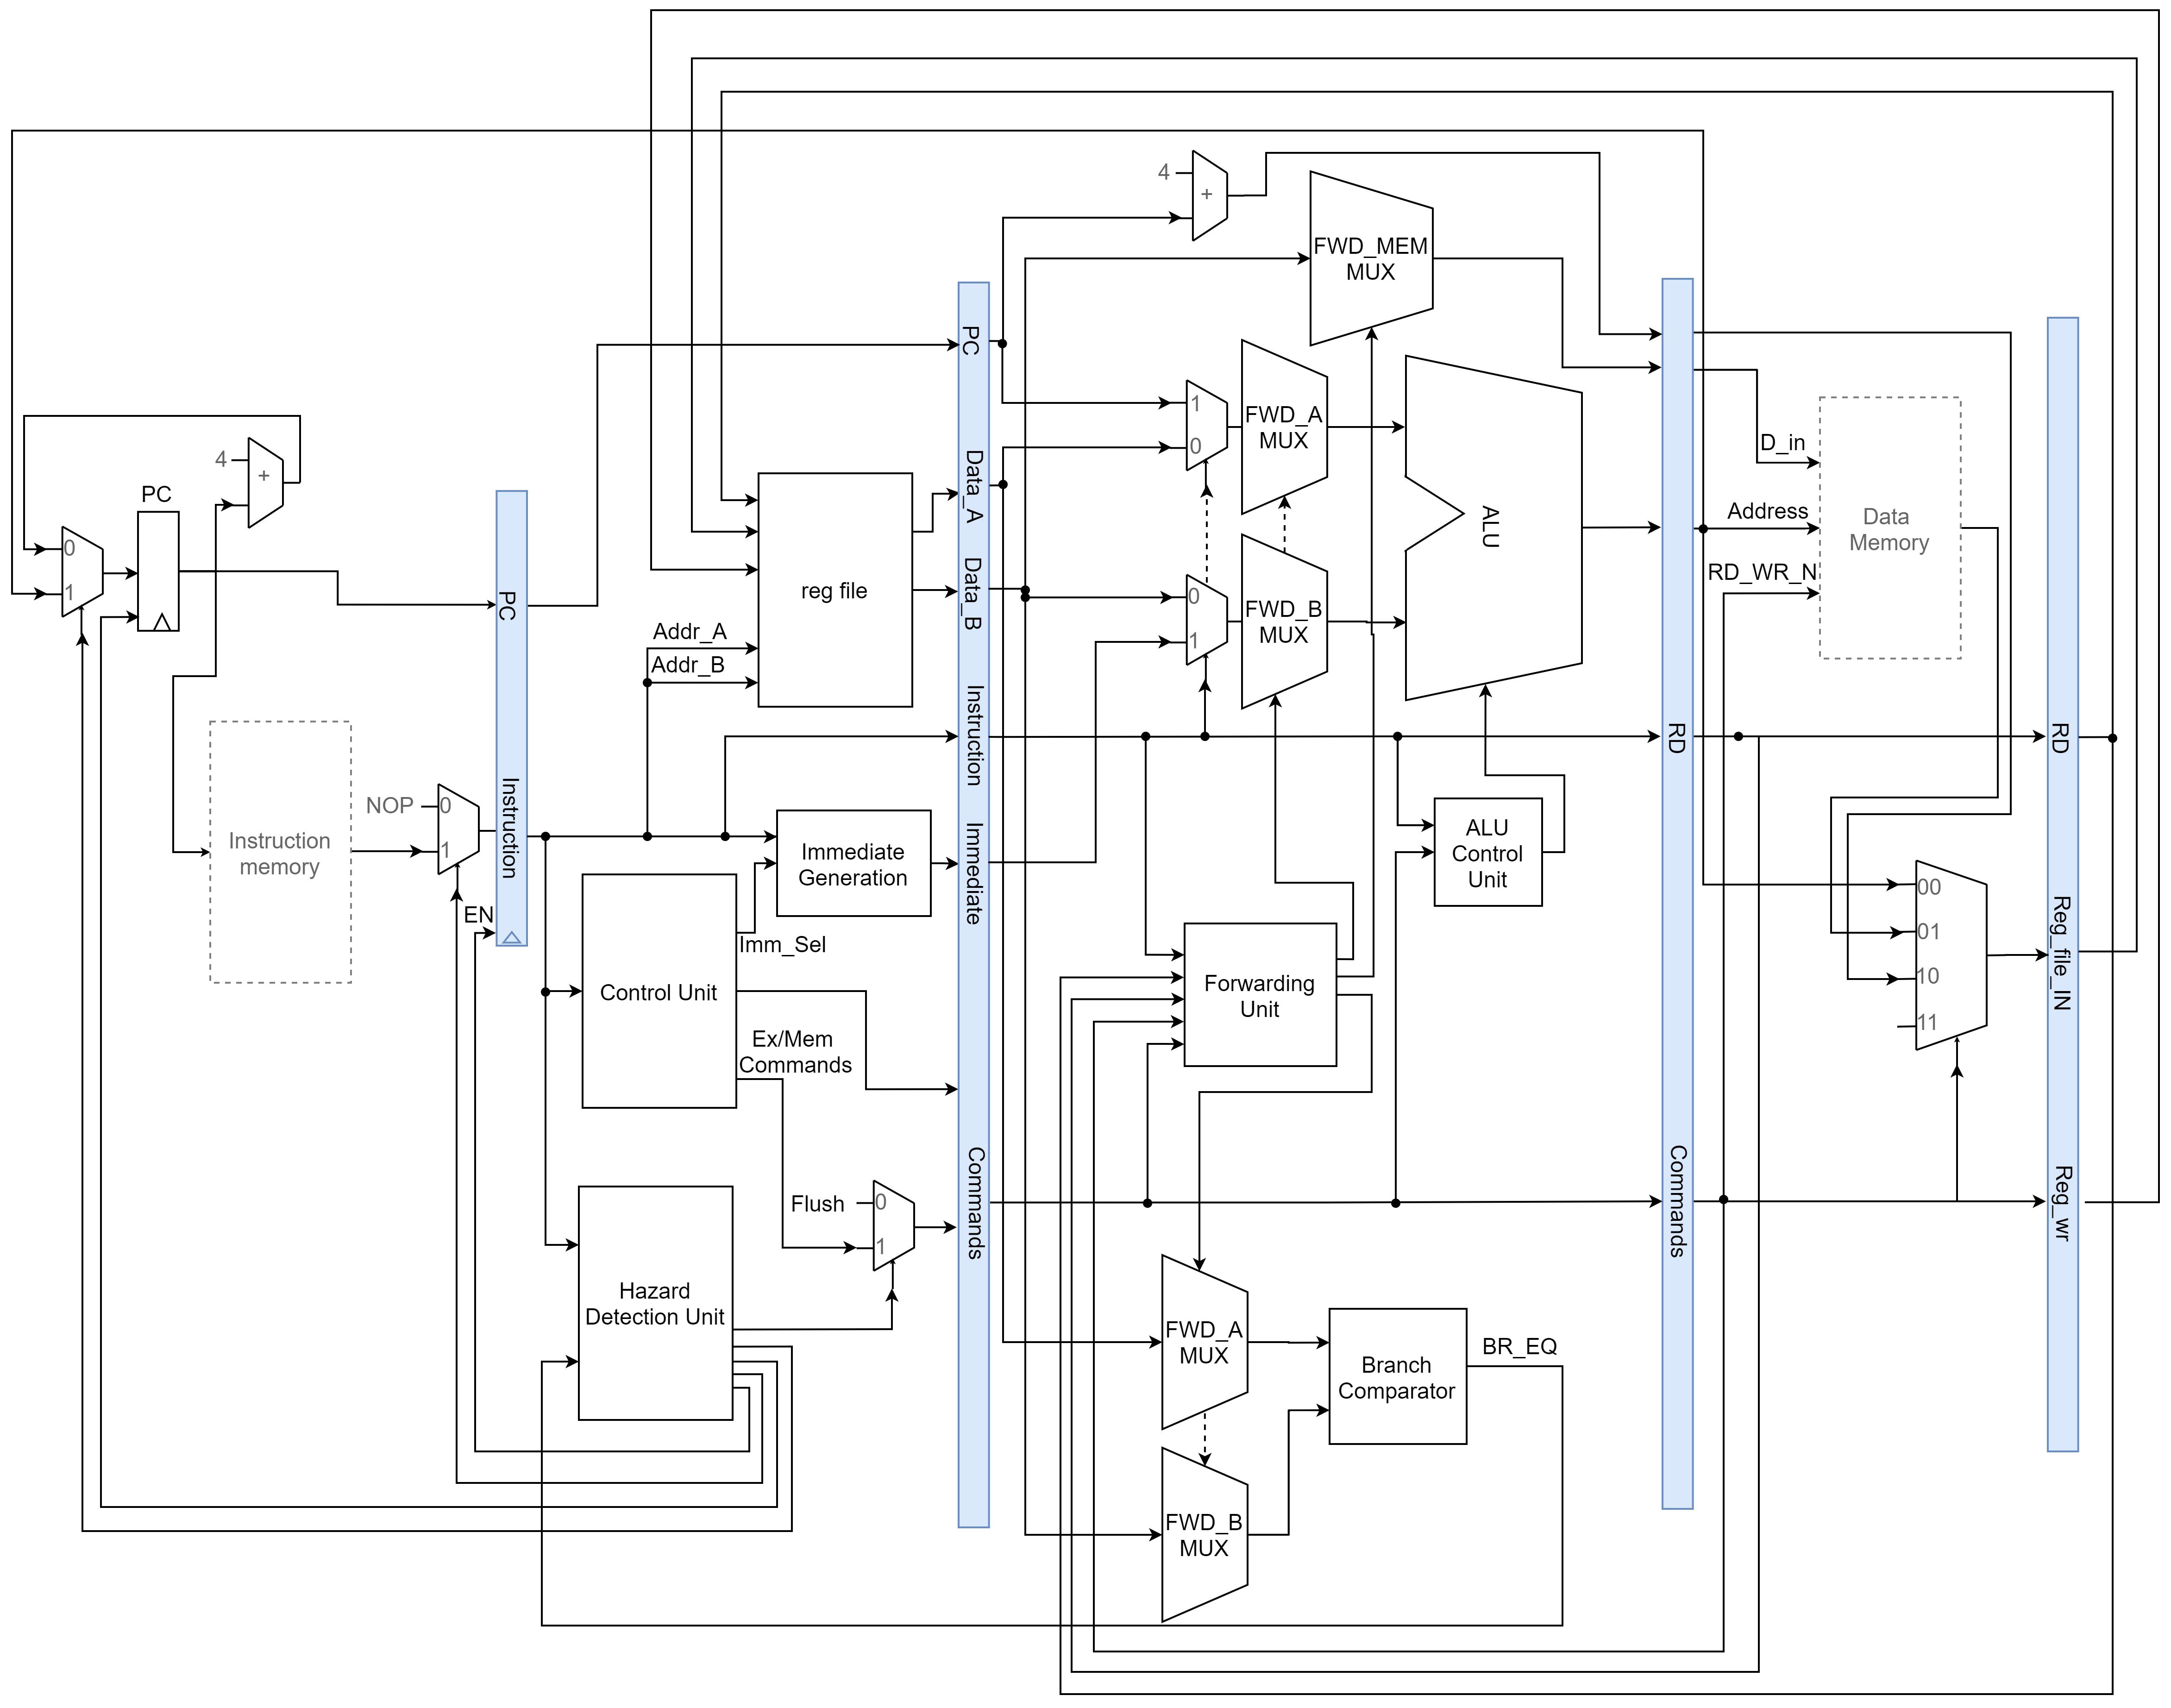
\includegraphics[width=1\textwidth]{sec2/images/datapath.png}
  \caption{Datapath architecture}
  \label{fig:datapath_architecture}
\end{figure}
